\section{Busybox}

\begin{frame}
  \frametitle{Why Busybox?}
  \begin{itemize}
  \item A Linux system needs a basic set of programs to work
    \begin{itemize}
    \item An init program
    \item A shell
    \item Various basic utilities for file manipulation and system
      configuration
    \end{itemize}
  \item In normal Linux systems, those programs are provided by
    different projects
    \begin{itemize}
    \item \code{coreutils}, \code{bash}, \code{grep}, \code{sed},
      \code{tar}, \code{wget}, \code{modutils}, etc. are all different
      projects
    \item A lot of different components to integrate
    \item Components not designed with embedded systems constraints in
      mind: they are not very configurable and have a wide range of
      features
    \end{itemize}
  \item Busybox is an alternative solution, extremely common on
    embedded systems
  \end{itemize}
\end{frame}

\begin{frame}
  \frametitle{General purpose toolbox: BusyBox}
  \begin{itemize}
  \item Rewrite of many useful Unix command line utilities
    \begin{itemize}
    \item Integrated into a single project, which makes it easy to
      work with
    \item Designed with embedded systems in mind: highly configurable,
      no unnecessary features
    \end{itemize}
  \item All the utilities are compiled into a single executable,
    \code{/bin/busybox}
    \begin{itemize}
    \item Symbolic links to \code{/bin/busybox} are created for each
      application integrated into Busybox
    \end{itemize}
  \item For a fairly featureful configuration, less than 500 KB
    (statically compiled with uClibc) or less than 1 MB (statically
    compiled with glibc).
  \item   \url{http://www.busybox.net/}
  \end{itemize}
\end{frame}

\begin{frame}
  \frametitle{BusyBox commands!}
  Commands available in BusyBox 1.13
  \begin{spacing}{0}
    \tiny
    \code{[, [[ , addgroup, adduser, adjtimex, ar, arp, arping, ash, awk, basename, bbconfig, bbsh, brctl, bunzip2, busybox, bzcat, bzip2, cal, cat, catv, chat, chattr, chcon, chgrp, chmod, chown, chpasswd, chpst, chroot, chrt, chvt, cksum, clear, cmp, comm, cp, cpio, crond, crontab, cryptpw, cttyhack, cut, date, dc, dd, deallocvt, delgroup, deluser, depmod, devfsd, df, dhcprelay, diff, dirname, dmesg, dnsd, dos2unix, dpkg, dpkg_deb, du, dumpkmap, dumpleases, e2fsck, echo, ed, egrep, eject, env, envdir, envuidgid, ether_wake, expand, expr, fakeidentd, false, fbset, fbsplash, fdflush, fdformat, fdisk, fetchmail, fgrep, find, findfs, fold, free, freeramdisk, fsck, fsck_minix, ftpget, ftpput, fuser, getenforce, getopt, getsebool, getty, grep, gunzip, gzip, halt, hd, hdparm, head, hexdump, hostid, hostname, httpd, hush, hwclock, id, ifconfig, ifdown, ifenslave, ifup, inetd, init, inotifyd, insmod, install, ip, ipaddr, ipcalc, ipcrm, ipcs, iplink, iproute, iprule, iptunnel, kbd_mode, kill, killall, killall5, klogd, lash, last, length, less, linux32, linux64, linuxrc, ln, load_policy, loadfont, loadkmap, logger, login, logname, logread, losetup, lpd, lpq, lpr, ls, lsattr, lsmod, lzmacat, makedevs, man, matchpathcon, md5sum, mdev, mesg, microcom, mkdir, mke2fs, mkfifo, mkfs_minix, mknod, mkswap, mktemp, modprobe, more, mount, mountpoint, msh, mt, mv, nameif, nc, netstat, nice, nmeter, nohup, nslookup, od, openvt, parse, passwd, patch, pgrep, pidof, ping, ping6, pipe_progress, pivot_root, pkill, poweroff, printenv, printf, ps, pscan, pwd, raidautorun, rdate, rdev, readahead, readlink, readprofile, realpath, reboot, renice, reset, resize, restorecon, rm, rmdir, rmmod, route, rpm, rpm2cpio, rtcwake, run_parts, runcon, runlevel, runsv, runsvdir, rx, script, sed, selinuxenabled, sendmail, seq, sestatus, setarch, setconsole, setenforce, setfiles, setfont, setkeycodes, setlogcons, setsebool, setsid, setuidgid, sh, sha1sum, showkey, slattach, sleep, softlimit, sort, split, start_stop_daemon, stat, strings, stty, su, sulogin, sum, sv, svlogd, swapoff, swapon, switch_root, sync, sysctl, syslogd, tac, tail, tar, taskset, tcpsvd, tee, telnet, telnetd, test, tftp, tftpd, time, top, touch, tr, traceroute, true, tty, ttysize, tune2fs, udhcpc, udhcpd, udpsvd, umount, uname, uncompress, unexpand, uniq, unix2dos, unlzma, unzip, uptime, usleep, uudecode, uuencode, vconfig, vi, vlock, watch, watchdog, wc, wget, which, who, whoami, xargs, yes, zcat, zcip}
  \end{spacing}
\end{frame}

\begin{frame}
  \frametitle{Applet highlight: Busybox init}
  \begin{itemize}
  \item Busybox provides an implementation of an \code{init} program
  \item Simpler than the init implementation found on desktop/server
    systems: no runlevels are implemented
  \item A single configuration file: \code{/etc/inittab}
    \begin{itemize}
    \item Each line has the form \code{<id>::<action>:<process>}
    \end{itemize}
  \item Allows to run services at startup, and to make sure that
    certain services are always running on the system
  \item See \code{examples/inittab} in Busybox for details on the
    configuration
  \end{itemize}
\end{frame}

\begin{frame}
  \frametitle{Applet highlight - BusyBox vi}
  \begin{itemize}
  \item If you are using BusyBox, adding \code{vi} support only adds
    20K. (built with shared libraries, using uClibc).
  \item You can select which exact features to compile in.
  \item Users hardly realize that they are using a lightweight \code{vi}
    version!
  \item Tip: you can learn \code{vi} on the desktop, by running the \code{vimtutor}
    command.
  \end{itemize}
\end{frame}

\begin{frame}
  \frametitle{Configuring BusyBox}
  \begin{itemize}
  \item Get the latest stable sources from \url{http://busybox.net}
  \item Configure BusyBox (creates a \code{.config} file):
    \begin{itemize}
    \item \code{make defconfig}\\
      Good to begin with BusyBox.\\
      Configures BusyBox with all options for regular users.
    \item \code{make allnoconfig}\\
      Unselects all options. Good to configure only what you need.
    \end{itemize}
  \item \code{make xconfig} (graphical, needs the \code{libqt3-mt-dev} package)\\
    or \code{make menuconfig} (text)\\
    Same configuration interfaces as the ones used by the Linux kernel
    (though older versions are used).
  \end{itemize}
\end{frame}

\begin{frame}
  \frametitle{BusyBox make xconfig}
  \begin{columns}
    \column{0.3\textwidth}
    You can choose:
    \begin{itemize}
    \item the commands to compile,
    \item and even the command options and features that you need!
    \end{itemize}
    \column{0.7\textwidth}
    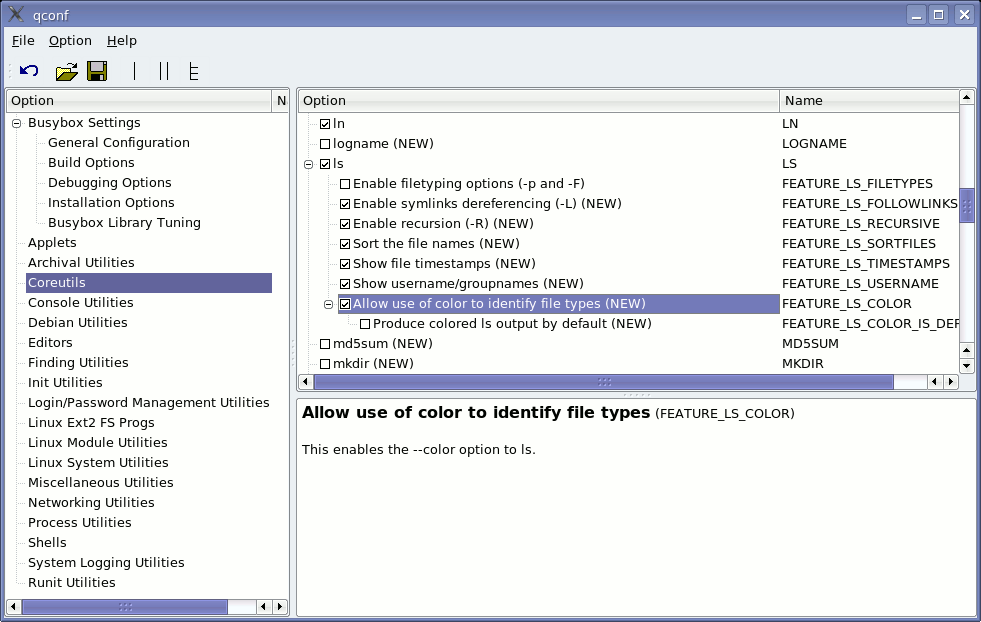
\includegraphics[width=\textwidth]{slides/sysdev-busybox/xconfig-screenshot.png}
  \end{columns}
\end{frame}

\begin{frame}
  \frametitle{Compiling BusyBox}
  \begin{itemize}
  \item Set the cross-compiler prefix in the configuration interface: \\
    \code{BusyBox Settings ->  Build Options ->  Cross Compiler
      prefix}\\
    Example: \code{arm-linux-}
  \item Set the installation directory in the configuration interface: \\
    \code{BusyBox Settings ->  Installation Options ->  BusyBox
      installation prefix}
  \item Add the cross-compiler path to the PATH environment variable:\\
    \code{export PATH=/usr/xtools/arm-unknown-linux-uclibcgnueabi/bin:$PATH}
  \item Compile BusyBox:\\
    \code{make}
  \item Install it (this creates a Unix directory structure symbolic
    links to the \code{busybox} executable):\\
    \code{make install}
  \end{itemize}
\end{frame}

\setuplabframe
{A tiny embedded system}
{
  \begin{itemize}
  \item Make Linux boot on a directory on your workstation, shared by NFS
  \item Create and configure a minimalistic Linux embedded system
  \item Install and use BusyBox
  \item System startup with \code{/sbin/init}
  \item Setup a simple web interface
  \item Use shared libraries
  \end{itemize}
}
